% Title: Example for tkz-orm v0.1 2010/01/25
% Author: Jakob Voß
% Site: http://tug.ctan.org/tex-archive/graphics/pgf/contrib/tkz-orm/
%
% This is an example for the 'tkz-orm' package included in its
% documentation. It redraws a diagram found in Halpin & Morgan's
% "Information modeling and relational databases" p 902.
\documentclass{article}
\usepackage{tkz-orm}
\begin{document}
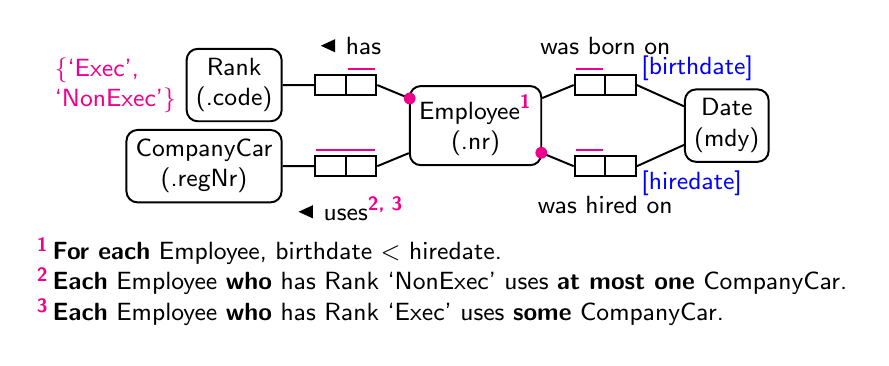
\begin{tikzpicture}[orm]
    \entity (E) {Employee\ormind{1}\\(.nr)};

    \binary[left=of E.north west, unique=2, label=\ormleft{has}] (h) {};
    \binary[left=of E.south west, unique=1-2,
         label=below:\ormleft{uses\ormind{2, 3}}] (u) {};

    \entity[left=of h] (Rank) {Rank\\(.code)};
    \entity[left=of u] (Car) {CompanyCar\\(.regNr)};
    \node[constraint=text, align=left, anchor=east] at (Rank.west)
        {$\{$`Exec',\\`NonExec'$\}$};

    \plays[mandatory] (E) to (h.east);
    \plays (h) to (Rank) (E) to (u.east) (u) to (Car);

    \binary[right=of E.north east, unique, label=was born on] (b) {};
    \binary[right=of E.south east, unique, label=below:was hired on] (i) {};

    \entity[right=1.8 of E] (Date) {Date\\(mdy)};

    \plays[mandatory] (E) to (b.west) (E) to (i.west);
    \plays (b.east) to (Date) (i.east) to (Date);

    \node[role name, anchor=south west] at (b.east) {[birthdate]};
    \node[role name, anchor=north west] at (i.east) {[hiredate]};

    \rules at (-.4, -2) {
        \node[rule=1] {{\ormbf For each} Employee, birthdate $<$ hiredate.};\\
        \node[rule=2] {
             {\ormbf Each} Employee {\ormbf who} has Rank `NonExec' uses
             {\ormbf at most one} CompanyCar.};\\
        \node[rule=3] {
             {\ormbf Each} Employee {\ormbf who} has Rank `Exec' uses
             {\ormbf some} CompanyCar.};\\
    };
\end{tikzpicture}
\end{document}